\documentclass{anstrans}
%%%%%%%%%%%%%%%%%%%%%%%%%%%%%%%%%%%
\title{Cerberus: A MOOSE-based application for solving the SP$_3$ equations}
\author{Roberto E. Fairhurst Agosta, Kathryn D. Huff}

\institute{
University of Illinois at Urbana-Champaign, Dept. of Nuclear, Plasma, and Radiological Engineering\\
ref3@illinois.edu
}

%%%% packages and definitions (optional)
\usepackage{graphicx} % allows inclusion of graphics
\usepackage{booktabs} % nice rules (thick lines) for tables
\usepackage{microtype} % improves typography for PDF
\usepackage{xspace}
\usepackage{tabularx}
\usepackage{caption}
\usepackage{floatrow}
\usepackage{subcaption}
\usepackage{enumitem}
\usepackage{placeins}
\usepackage{amsmath}
\usepackage[acronym,toc]{glossaries}
\newacronym{ANL}{ANL}{Argonne National Laboratory}
\newacronym{API}{API}{Application Programming Interface}
\newacronym{B4C}{B4C}{boron carbide}
\newacronym{BC}{BC}{boundary condition}
\newacronym{BOC}{BOC}{beginning of the equilibrium cycle}
\newacronym{BSD}{BSD}{Berkeley Software Distribution}
\newacronym{BWR}{BWR}{Boiling Water Reactor}
\newacronym{CAISO}{CAISO}{California ISO}
\newacronym{CAPP}{CAPP}{Core Analyzer for Pebble and Prism type VHTRs}
\newacronym{CEA}{CEA}{Commissariat a l'Energie Atomique}
\newacronym{CFD}{CFD}{computational fluid dynamics}
\newacronym{CO2}{CO$_2$}{carbon dioxide}
\newacronym{CR}{CR}{control rod}
\newacronym{CRP}{CRP}{Coordinated Research Project}
\newacronym{CZP}{CZP}{Cold Zero Power}
\newacronym{DCC}{DCC}{depressurized conduction cool-down}
\newacronym{DOE}{DOE}{Department of Energy}
\newacronym[\glslongpluralkey={degrees of freedom}]{DoF}{DoF}{degree of freedom}
\newacronym{EOC}{EOEC}{end of the equilibrium cycle}
\newacronym{FCEV}{FCEV}{Fuel Cell Electric Vehicle}
\newacronym{FDM}{FDM}{Finite Difference Method}
\newacronym{FEM}{FEM}{Finite Element Method}
\newacronym{FVM}{FVM}{Finite Volume Method}
\newacronym[\glslongpluralkey={greenhouse gases}]{GHG}{GHG}{greenhouse gas}
\newacronym{GRS}{GRS}{Gesellschaft für Anlagen und Reaktorsicherheit}
\newacronym{GT-MHR}{GT-MHR}{Gas Turbine-Modular Helium Reactor}
\newacronym{H2}{H$_2$}{hydrogen}
\newacronym{He}{He}{helium}
\newacronym{HFP}{HFP}{Hot Full Power}
\newacronym{HPCC}{HPCC}{high-pressure conduction cool-down}
\newacronym{HTE}{HTE}{High-Temperature Electrolysis}
\newacronym{HTGR}{HTGR}{High-Temperature Gas-Cooled Reactor}
\newacronym{HTR}{HTR}{High Temperature Reactor}
\newacronym{HTTR}{HTTR}{High-Temperature engineering Test Reactor}
\newacronym{HZDR}{HZDR}{Helmholtz-Zentrum Dresden-Rossendorf}
\newacronym{IAEA}{IAEA}{International Atomic Energy Agency}
\newacronym{icap}{iCAP}{Illinois Climate Action Plan}
\newacronym{INL}{INL}{Idaho National Laboratory}
\newacronym{IPyC}{IPyC}{inner pyrolytic carbon}
\newacronym{JFNK}{JFNK}{Jacobian-Free Newton-Krylov}
\newacronym{KAERI}{KAERI}{Korea Atomic Energy Research Institute}
\newacronym{Keff}{k$_{eff}$}{multiplication factor}
\newacronym{LBP}{LBP}{Lumped Burnable Poison}
\newacronym{LGPL}{LGPL}{Lesser GNU Public License}
\newacronym{LOCA}{LOCA}{loss of coolant accident}
\newacronym{LPCC}{LPCC}{low-pressure conduction cool-down}
\newacronym{LTE}{LTE}{Low-Temperature Electrolysis}
\newacronym{LWR}{LWR}{Light Water Reactor}
\newacronym{MC}{MC}{Monte Carlo}
\newacronym{MHTGR}{MHTGR}{Modular High-Temperature Gas-Cooled Reactor}
\newacronym{MMR}{MMR}{Micro Modular Reactor}
\newacronym{MOC}{MOC}{middle of the equilibrium cycle}
\newacronym{MOX}{MOX}{mixed-oxide}
\newacronym{MOOSE}{MOOSE}{Multi-physics Object-Oriented Simulation Environment}
\newacronym{MPI}{MPI}{Message Passing Interface}
\newacronym{MSR}{MSR}{Molten Salt Reactor}
\newacronym{MTD}{MTD}{Champaign-Urbana Mass Transit District}
\newacronym{NEA}{NEA}{Nuclear Energy Agency}
\newacronym{NEM}{NEM}{Nodal Expansion Method}
\newacronym{NGNP}{NGNP}{Next Generation Nuclear Power}
\newacronym{NRC}{NRC}{Nuclear Regulatory Commission}
\newacronym{NSC}{NSC}{Nuclear Science Committee}
\newacronym{OECD}{OECD}{Organisation for Economic Co-operation and Development}
\newacronym{OPyC}{OPyC}{outer pyrolytic carbon}
\newacronym{ORNL}{ORNL}{Oak Ridge National Laboratory}
\newacronym{OS}{OS}{Operator-Splitting}
\newacronym{PBMR}{PBMR}{Pebble Bed Modular Reactor}
\newacronym{PDE}{PDE}{Partial Differential Equation}
\newacronym{PMR}{PMR}{Prismatic Modular Reactor}
\newacronym{PV}{PV}{photovoltaics}
\newacronym{RPV}{RPV}{Reactor Pressure Vessel}
\newacronym{RSC}{RSC}{Reserve Shutdown Control}
\newacronym{RSD}{RSD}{Relative Standard Deviation}
\newacronym{SD}{SD}{Standard Deviation}
\newacronym{SI}{SI}{Sulfur-Iodine}
\newacronym{SiC}{SiC}{silicon carbide}
\newacronym{SMR}{SMR}{Small Modular Reactor}
\newacronym{SNU}{SNU}{Seoul National University}
\newacronym{SOEC}{SOEC}{Solid Oxide Electrolysis Cells}
\newacronym{SP3}{SP$_3$}{Simplified P$_3$}
\newacronym{TIP}{TIP}{transverse integration procedure}
\newacronym{TRISO}{TRISO}{Tristructural Isotropic}
\newacronym{UIUC}{UIUC}{University of Illinois at Urbana-Champaign}
\newacronym{UNIST}{UNIST}{Ulsan National Institute of Science and Technology}
\newacronym{UK}{UK}{United Kingdom}
\newacronym{UMICH}{UMICH}{University of Michigan}
\newacronym{US}{US}{United States}
\newacronym{USNC}{USNC}{Ultra Safe Nuclear Corporation}
\newacronym{VHTR}{VHTR}{Very High-Temperature Gas-Cooled Reactor}
%\newacronym{<++>}{<++>}{<++>}
%\newacronym{<++>}{<++>}{<++>}

\makeglossaries

\usepackage[printwatermark]{xwatermark}
\usepackage{xcolor}
\usepackage{graphicx}
\usepackage{lipsum}

\newcommand{\SN}{S$_N$}
\renewcommand{\vec}[1]{\bm{#1}} %vector is bold italic
\newcommand{\vd}{\bm{\cdot}} % slightly bold vector dot
\newcommand{\grad}{\vec{\nabla}} % gradient
\newcommand{\ud}{\mathop{}\!\mathrm{d}} % upright derivative symbol

\newcolumntype{c}{>{\hsize=.56\hsize}X}
\newcolumntype{b}{>{\hsize=.7\hsize}X}
\newcolumntype{s}{>{\hsize=.74\hsize}X}
\newcolumntype{f}{>{\hsize=.1\hsize}X}
\newcolumntype{a}{>{\hsize=.45\hsize}X}
%\usepackage[pagestyles]{titlesec}
%\titleformat*{\subsection}{\normalfont}
%\titleformat{\section}{\bfseries}{Item \thesection.\ }{0pt}{}

%\newwatermark[allpages,color=gray!50,angle=45,scale=3,xpos=0,ypos=0]{DRAFT}

\begin{document}
%%%%%%%%%%%%%%%%%%%%%%%%%%%%%%%%%%%%%%%%%%%%%%%%%%%%%%%%%%%%%%%%%%%%%%%%%%%%%%%%

% \section{Abstract}

% \textit{
%     The Multi-physics Object-Oriented Simulation Environment is a framework that supports the development of applications for solving nonlinear systems of differential equations.
%     This work presents the implementation of an application in that framework for solving the Simplified $P_3$ equations.
%     We conducted two exercises with results as low as 12 pcm and as high as 145 pcm from the reference results, successfully validating the proposed application.
% }

\section{Introduction}

% what I am doing
This work presents the implementation of the Simplified P$_3$ (SP$_3$) equations \cite{gelbard_spherical_1960} in the \gls{MOOSE}-based application Cerberus.
% MOOSE
MOOSE \cite{gaston_moose_2009} is a computational framework that supports engineering analysis applications.
In a nuclear reactor, several partial differential equations describe its physical behavior.
These equations are typically nonlinear, and they are often coupled to each other.
MOOSE is an open-source \gls{FEM} framework that supports the development of applications for solving such systems.

% MOOSE supports the development of applications for solving such systems.
% MOOSE is an open-source \gls{FEM} framework.
% The framework itself relies on LibMesh \cite{kirk_libmesh_2006} and PetSc \cite{balay_petsc_2016} for solving nonlinear equations.
% MOOSE-based applications define weak forms of the governing equations and modularize the physics expressions into "kernels."
% Kernels are C++ classes containing methods for computing the residual and Jacobian contributions of individual pieces of the governing equations.
% MOOSE and LibMesh translate them into residual and Jacobian functions.
% These functions become inputs into PetSc solution routines.

All the software built on the MOOSE framework shares the same \gls{API}, facilitating relatively easy coupling between different phenomena.
While Cerberus solves the neutronics in a nuclear reactor using the multi-group steady-state SP$_3$ equations, other applications may solve the thermal-fluids, and given they share the same API; their integration is straightforward.
% Additionally, the framework and its applications use \gls{MPI} for parallel communication allowing for deployment on massively-parallel cluster-computing platforms.

% lit - review: the SPN approximation
The P$_N$ method \cite{davidson_neutron_1957} discretizes the transport equation by expanding the angular dependence of the neutron flux in spherical harmonics, considering up to order $N$ polynomials.
If $N \rightarrow \infty$, the solution of the P$_N$ equations tends to the exact transport solution.
In three-dimensional geometries, the number of P$_N$ equations is proportional to $(N+1)^2$, whereas, in one-dimensional planar geometries, the number of P$_N$ equations is $(N+1)$.
Gelbard \cite{gelbard_spherical_1960} proposed the SP$_N$ approximation by replacing the second derivatives in the one-dimensional planar P$_N$ equations with three-dimensional Laplacian operators.
This approximation considerably reduces the number of equations conserving a reasonable accuracy \cite{capilla_applications_2009}.
% Capilla et al. \cite{capilla_applications_2009} studied a modified version of the C5 \gls{MOX} fuel Benchmark \cite{cavarec_benchmark_1994} introduced by Brantley and Larsen \cite{brantley_simplifiedP3_2000} comparing the $P_3$ and $SP_3$ methods, the difference between results being less than 40 pcm.

The SP$_N$ approximation has the disadvantage that the solution does not usually converge to the true transport solution as $N \rightarrow \infty$.
Additionally, the theoretical basis of Gelbard's formulation of SP$_N$ approximation was weak.
For these reasons, the method did not gain widespread use until the 2000s, when thanks to Pomraning \cite{pomraning_asymptotic_1993}, Brantley, and Larsen's \cite{brantley_simplifiedP3_2000} contribution, the method gained a stronger theoretical basis.
% Although Gelbard proposed the $SP_N$ approximation in the 60s, the method did not have a strong theoretical basis until the 90s with Pomraning \cite{pomraning_asymptotic_1993}, Brantley, and Larsen's \cite{brantley_simplifiedP3_2000} contribution.
% Additionally, the $SP_N$ approximation has the disadvantage that the solution does not usually converge to the true transport solution as $N \rightarrow \infty$.

In practice, the SP$_N$ equations are most accurate for diffusive problems or for problems in which the solution behaves nearly one-dimensionally and has weak tangential derivatives at material interfaces.
% For problems with strong, multidimensional transport effects, such as voids, streaming regions, or geometrically complex regions, the $SP_N$ solutions are less accurate \cite{downar_parcs_2004}.
% However, several results show that the $SP_N$ approximation yields more accurate solutions than the diffusion approximation \cite{mui_modified_1987} \cite{beckert_development_2007} \cite{fliscounakis_potential_2012} \cite{ryu_finite_2013} \cite{khosravi_mirzaee_reactor_2019} with considerably less computational expense than the discrete ordinates ($S_N$) method \cite{brantley_simplifiedP3_2000}.
Several results show that the SP$_N$ approximation yields more accurate solutions than the diffusion approximation \cite{mui_modified_1987} \cite{beckert_development_2007} \cite{fliscounakis_potential_2012} \cite{ryu_finite_2013} with considerably less computational expense than the discrete ordinates ($S_N$) method \cite{brantley_simplifiedP3_2000}.
% why is SP_3 preferred over diffusion
For example, the SP$_3$ approximation is preferable over the diffusion approximation for modeling reactors using MOX/UO$_2$ fuel assemblies.
MOX fuel assemblies have higher thermal absorption and fission cross-sections than UO$_2$ fuel assemblies, and consequently, their thermal flux is lower while their power production higher.
Modeling these characteristics using the diffusion approximation may be challenging \cite{brantley_simplifiedP3_2000} \cite{capilla_applications_2009}.

% lit - review: software using the SPN approximation
The SP$_3$ approximation gained usage throughout the last couple of decades and currently, different software uses it to solve the neutron transport equation.
% Some of those software are SCOPE2 \cite{tatsumi_object-oriented_2002}, PARCS \cite{downar_parcs_2004}, DYN3D \cite{beckert_development_2007}, SIMULATE-5 \cite{bahadir_studsviks_2009}, and COCAGNE \cite{fliscounakis_potential_2012}.
Some of those software are PARCS \cite{downar_parcs_2004}, DYN3D \cite{beckert_development_2007}, and COCAGNE \cite{fliscounakis_potential_2012}.

\section{Methodology}

This section describes the methodology followed for solving the equations.
% Equations P3
Davidson \cite{davidson_neutron_1957} defined the one-dimensional multi-group P$_N$ equations.
In the steady state, and for $N=3$, the equations become

\begin{align}
    & \frac{d}{dx} \phi_{1,g} + \Sigma_{t,g} \phi_{0,g} = \sum_{g'=1}^G \Sigma_{s0,g' \rightarrow g} \phi_{0,g'} + \frac{\chi_g}{k_{eff}} \sum_{g'=1}^G \nu\Sigma_{f,g'} \phi_{0,g'} \notag \\ & \quad \quad \quad \quad \quad \quad \quad + Q_{0,g}  \label{eq:P3-0} \\
    & \frac{1}{3} \frac{d}{dx} \phi_{0,g} + \frac{2}{3}\frac{d}{dx}\phi_{2,g} + \Sigma_{t,g} \phi_{1,g} = \sum_{g'=1}^G \Sigma_{s1,g' \rightarrow g} \phi_{1,g'} + Q_{1,g} \label{eq:P3-1} \\
    & \frac{2}{5} \frac{d}{dx}\phi_{1,g} + \frac{3}{5}\frac{d}{dx}\phi_{3,g} + \Sigma_{t,g} \phi_{2,g} = \sum_{g'=1}^G \Sigma_{s2,g' \rightarrow g} \phi_{2,g'} + Q_{2,g} \label{eq:P3-2} \\
    & \frac{3}{7}\frac{d}{dx}\phi_{2,g} + \Sigma_{t,g} \phi_{3,g} = \sum_{g'=1}^G \Sigma_{s3,g' \rightarrow g} \phi_{3,g'} + Q_{3,g} \label{eq:P3-3} \\
    \intertext{where}
    & \phi_{n,g} = \mbox{$n^{th}$ moment of group $g$ neutron flux}  \notag \\ %  } [n \cdot cm^{-2} \cdot s^{-1}]
    & \Sigma_{t,g} = \mbox{group $g$ macroscopic total cross-section}  \notag \\ %  } [cm^{-1}]
	& \Sigma_{sn,g' \rightarrow g} = \mbox{$n^{th}$ moment of the group $g'$ to group $g$} \notag \\
	& \mbox{macroscopic scattering cross-section}  \notag \\ %  } [cm^{-1}]
	& \nu\Sigma_{f,g} = \mbox{group $g$ macroscopic production cross-section}  \notag \\ %  } [cm^{-1}]
	& \chi_{g} = \mbox{group $g$ fission spectrum}  \notag \\ %  } [cm^{-1}]
	& k_{eff} = \mbox{eigenvalue}  \notag \\ %  } [-]
	& Q_{n,g} = \mbox{$n^{th}$ moment of group $g$ external neutron source}  \notag \\  % } [n \cdot cm^{-3} \cdot s^{-1}]
	& G = \mbox{number of energy groups}.  \notag % } [-]
\end{align}

Assuming an isotropic external source and negligible anisotropic group-to-group scattering \cite{brantley_simplifiedP3_2000}
\begin{align}
	& Q_{n,g} = 0, \quad n > 0 \notag \\
	& \Sigma_{sn,g' \rightarrow g} = 0, \quad g' \ne g, \quad n > 0 \notag
\end{align}

\noindent
simplifies equations \ref{eq:P3-1} and \ref{eq:P3-3}, allowing to express the odd moments of the flux $\phi_{1,g}$ and $\phi_{3,g}$ as functions of the even moments $\phi_{0,g}$ and $\phi_{2,g}$.
Replacing $\phi_{1,g}$ and $\phi_{3,g}$ into equations \ref{eq:P3-0} and \ref{eq:P3-2} reduces the system from four to two equations.
Introducing the variables $\Phi_{0,g}$ and $\Phi_{2,g}$, reorganizing the equations, and replacing the second derivatives by Laplacian operators \cite{gelbard_spherical_1960} yields the SP$_3$ equations \cite{beckert_development_2007}

% Equations SP_3
\begin{align}
    & - D_{0,g} \Delta \Phi_{0,g} + \Sigma_{0,g} \Phi_{0,g} - 2 \Sigma_{0,g} \Phi_{2,g} = S_{0,g} \label{eq:SP3-0e} \\
    & - D_{2,g} \Delta \Phi_{2,g} + \left( \Sigma_{2,g} + \frac{4}{5} \Sigma_{0,g} \right) \Phi_{2,g} - \frac{2}{5} \Sigma_{0,g} \Phi_{0,g} = -\frac{2}{5} S_{0,g} \label{eq:SP3-2e}
    \intertext{where}
	& \Sigma_{n,g} = \Sigma_{t,g} - \Sigma_{sn,g' \rightarrow g} \notag \\
    & \Phi_{0,g} = \phi_{0,g} + 2 \phi_{2,g} \notag \\
    & \Phi_{2,g} = \phi_{2,g} \notag \\
    & D_{0,g} = \frac{1}{3 \Sigma_{1,g}} \label{eq:diff-rem} \\
    & D_{2,g} = \frac{9}{35 \Sigma_{3,g}} \notag \\
    & S_{0,g} = \sum_{g'\ne g}^G \Sigma_{s0,g' \rightarrow g} \left( \Phi_{0,g'} - 2 \Phi_{2,g'} \right) \notag \\
    & \quad \quad + \frac{\chi_g}{k_{eff}} \sum_{g'=1}^G \nu\Sigma_{f,g'} \left( \Phi_{0,g'} - 2 \Phi_{2,g'} \right) + Q_{0,g}. \notag
\end{align}

% BCs
The Marshak-like vacuum \glspl{BC} complete the system of equations \cite{beckert_development_2007}

\begin{align}
    & \frac{1}{4} \Phi_{0,g} \pm \frac{1}{2} \hat{n} \cdot J_{0,g} - \frac{3}{16} \Phi_{2,g} = 0 \label{eq:SP3-BC1a} \\
    - & \frac{3}{80} \Phi_{0,g} \pm \frac{1}{2} \hat{n} \cdot J_{2,g} + \frac{21}{80} \Phi_{2,g} = 0 \label{eq:SP3-BC2a}
    \intertext{where}
    & J_{n,g} = -D_{n,g} \nabla \Phi_{n,g}. \notag
\end{align}

Finally, multiplying equations \ref{eq:SP3-0e} and \ref{eq:SP3-2e} by a test function and integrating over the domain yields the weak form of the equations modularized into kernels by Cerberus.
For brevity, we will not display the derivation of the kernels here.
Such procedure is standard in weighted residual methods and can be found in \cite{ryu_finite_2013} or any finite elements book \cite{quarteroni_numerical_1994}.


\section{Results}

This section presents several numerical results that validate Cerberus' calculation scheme.
The following sections discuss the results of a one group exercise presented in \cite{brantley_simplifiedP3_2000} and describe the results of the C5 MOX Benchmark \cite{cavarec_benchmark_1994}.

\subsection{One group two-dimensional problem}

This section describes a one group, isotropic-scattering eigenvalue problem introduced by Brantley and Larsen \cite{brantley_simplifiedP3_2000}.
This section also presents the eigenvalue obtained with Cerberus and compares it against the reference value.
Figure \ref{fig:2D} shows the problem's geometry, and Table \ref{tab:cross-sections} specifies its cross-sections.
Due to the problem's symmetry, the model included only a quarter of the core.
Using the \textit{Gmsh} \cite{geuzaine_gmsh_2009} meshing tool, we created the mesh, which had $6 \times 10^{3}$ elements.
The simulation convergence criterion was $10^{-8}$ for the neutron flux.

\begin{figure}[H] %or H 
    \centering
    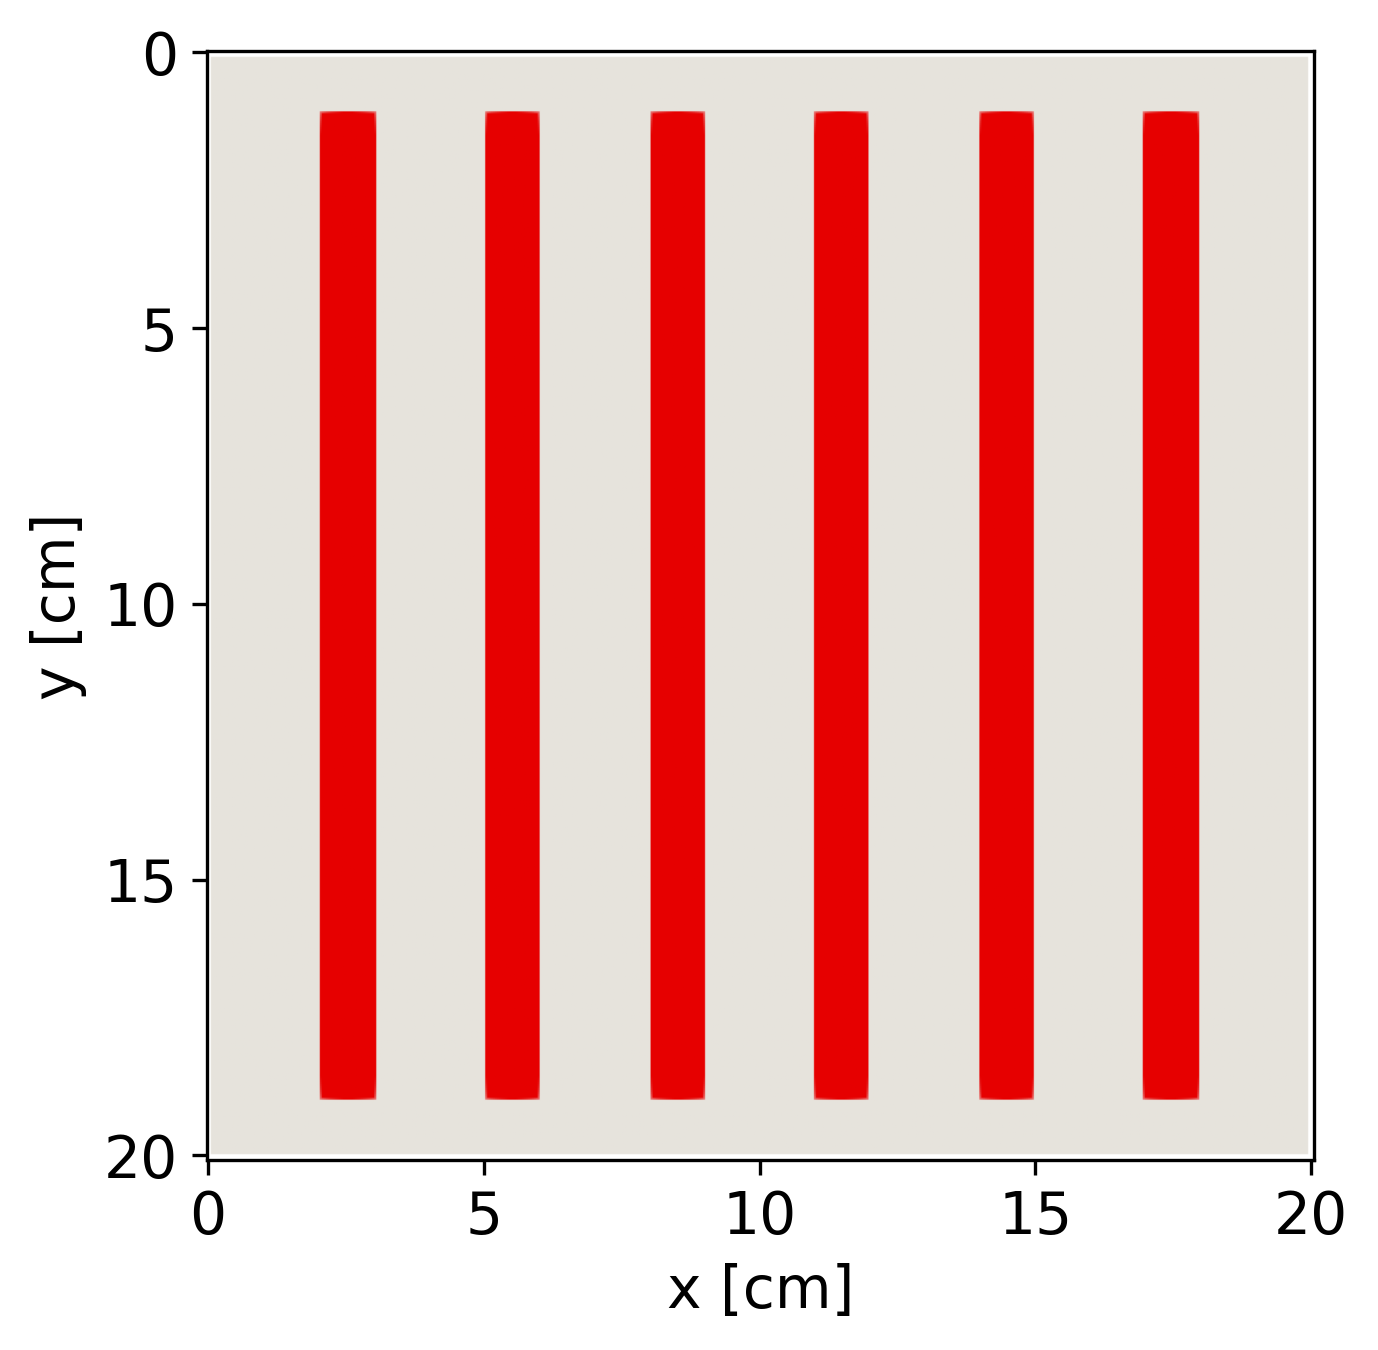
\includegraphics[width=0.75\linewidth]{figures/mesh2.png}
    \hfill
    \caption{Geometry of the one group eigenvalue problem. Fuel in red. Moderator in gray.}
    \label{fig:2D}
\end{figure}

% \usepackage{booktabs}
% \begin{table}[htbp!]
\begin{table}[h]
	\centering
	\caption{Cross-sections of the one group eigenvalue problem \cite{brantley_simplifiedP3_2000}. Values expressed in $cm^{-1}$.}
	\label{tab:cross-sections}
	\begin{tabular}{llll}
	\toprule
	Material	& $\Sigma_t$ & $\Sigma_{s0}$ & $\nu\Sigma_f$ \\
	\midrule
	Moderator	& 1.00		& 0.93			& 0.00			\\
	Fuel		& 1.50		& 1.35			& 0.24			\\
	\bottomrule
	\end{tabular}
\end{table}

Table \ref{tab:keff-1st} compares the eigenvalue obtained with the SP$_3$ solver and the reference value \cite{brantley_simplifiedP3_2000} using the equation
\begin{align}
  % & \Delta_\rho = \left| \rho_{SP_3} - \rho_{Ref} \right| = \left| \frac{k_{SP_3}-1}{k_{SP_3}} - \frac{k_{Ref}-1}{k_{Ref}} \right| = \left| \frac{k_{SP_3}-k_{Ref}}{k_{SP_3} k_{Ref}} \right| \label{eq:delta-rho} \\
  & \Delta_\rho = \left| \frac{k_{SP_3}-k_{Ref}}{k_{SP_3} k_{Ref}} \right| \label{eq:delta-rho} \\
  \intertext{where}
  & \Delta_\rho = \mbox{reactivity difference } [pcm] \notag \\
  & k_{SP_3} = \mbox{eigenvalue obtained with Cerberus} \notag \\
  & k_{Ref} = \mbox{reference eigenvalue.} \notag
\end{align}

\begin{table}[htbp!]
	\centering
	\caption{Comparison between the result obtained with Cerberus and the reference result for the one group eigenvalue problem.}
	\label{tab:keff-1st}
	\begin{tabular}{lll}
	\toprule
		$k_{Ref}$	& $k_{SP_3}$ 	& $\Delta_{\rho}$	\\
	\midrule
	 	0.79862		& 0.79854		& 12				\\
	\bottomrule
	\end{tabular}
\end{table}


\subsection{C5G2 2D Benchmark}

% intro to the benchmark
The open literature describes different versions and extensions of the C5 MOX benchmark, originally introduced by Cavarec et al. in 1994 \cite{cavarec_benchmark_1994}.
The \gls{OECD}/\gls{NEA} developed this benchmark to validate methods and identify their strengths, limitations, and accuracy, and suggest needs for method development.
This section describes the benchmark exercise and presents Cerberus results.

% benchmark specification
Two types of fuel assembly (MOX and UO$_2$) and a reflector comprise the core, shown in Figure \ref{fig:bench1}.
Each fuel assembly consists of a 17 $\times$ 17 array of squared pin cells, as displayed in Figures \ref{fig:bench2} and \ref{fig:bench3}.
The dimensions of each pin cell are 1.26 $\times$ 1.26 cm, being 21.42 $\times$ 21.42 cm the dimensions of each assembly, and 128.52 $\times$ 128.52 cm of the whole core.
The benchmark \cite{cavarec_benchmark_1994} specifies the cross-sections, which have a two-energy group structure.

\begin{figure}[htbp!] %or H 
    \centering
    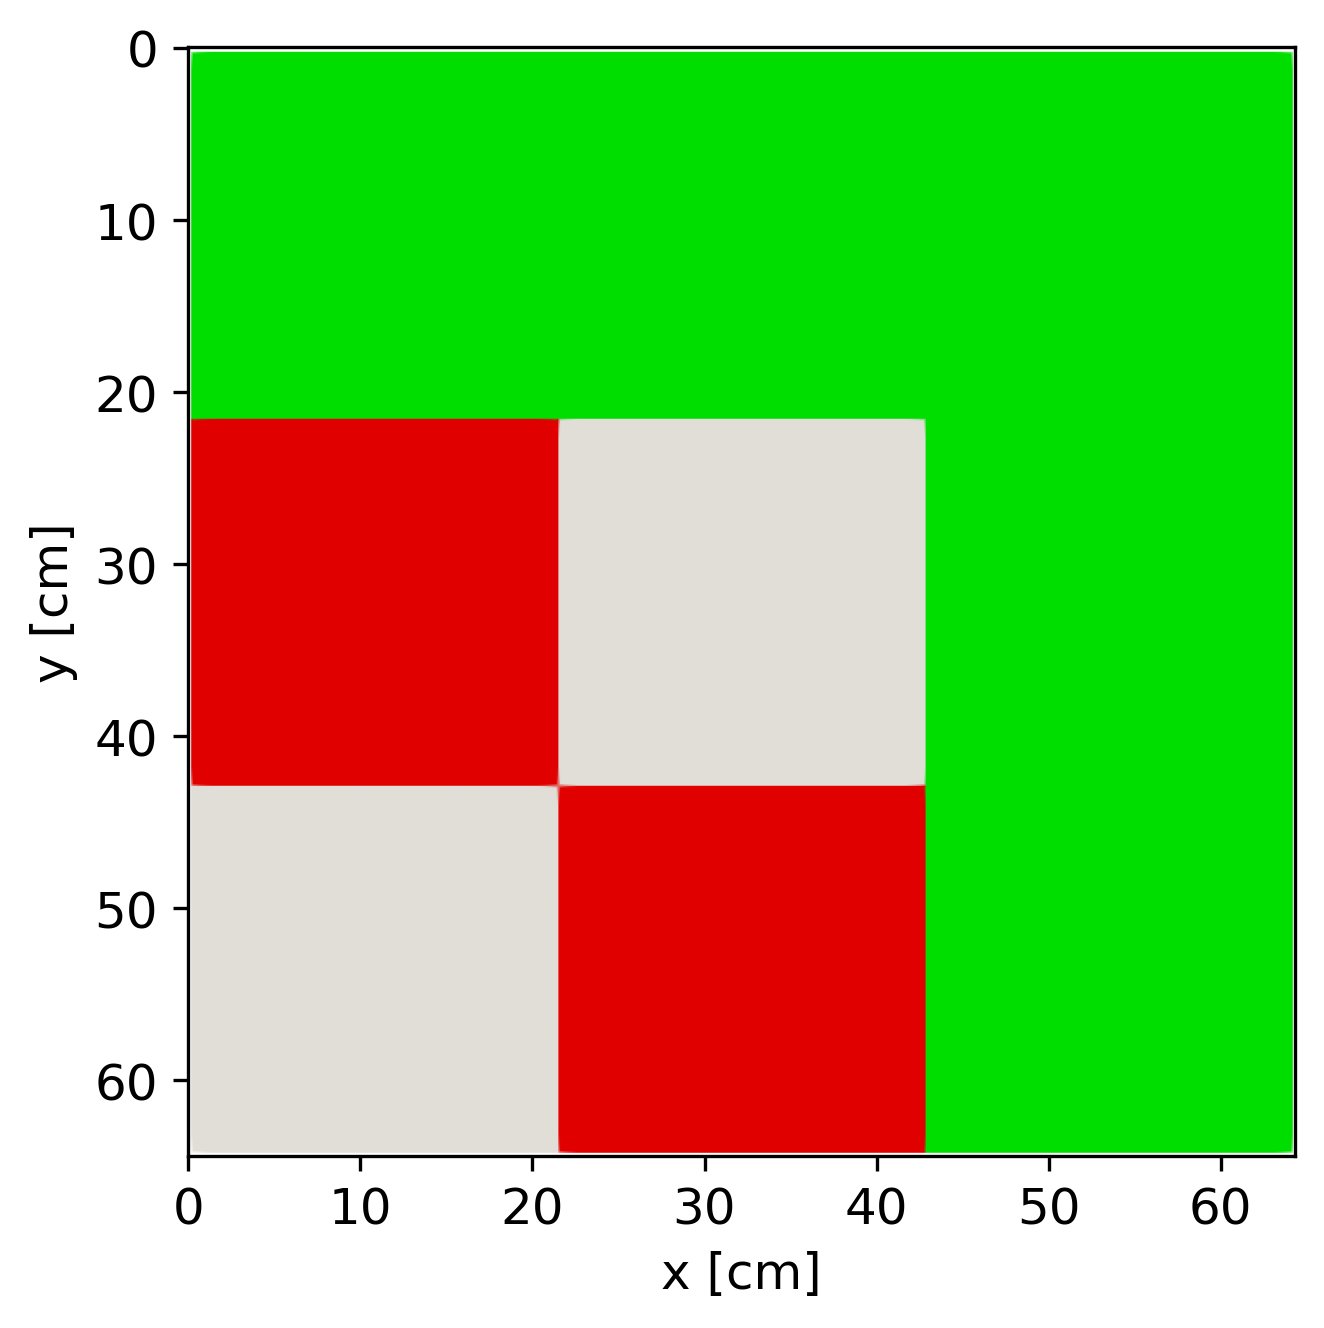
\includegraphics[width=0.85\linewidth]{figures/geo-xy2.png}
    \hfill
    \caption{C5 MOX benchmark configuration. UO$_2$ in gray. MOX in red. Reflector in green.}
    \label{fig:bench1}
\end{figure}

\begin{figure}[htbp!] %or H 
    \centering
    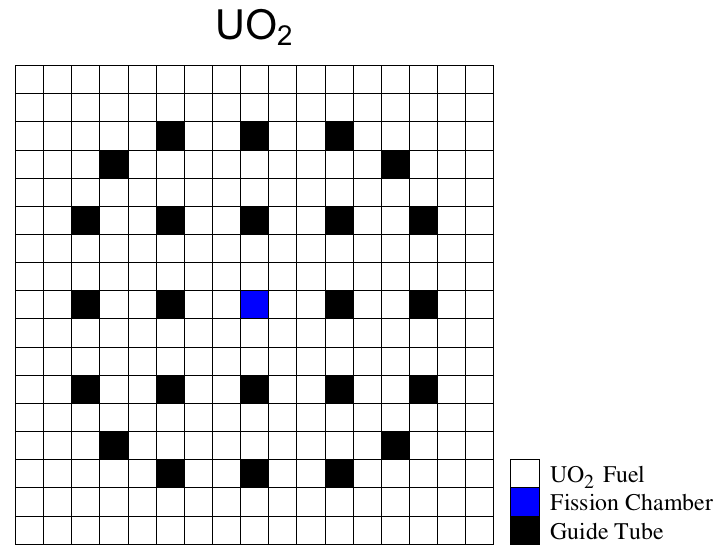
\includegraphics[trim=0 0 0 2.1cm, clip=true, width=0.85\linewidth]{figures/bench-config2.png}
    \hfill
    \caption{Structure of the UO$_2$ assembly. Image reproduced from \cite{capilla_applications_2009}.}
    \label{fig:bench2}
\end{figure}

When no anisotropic component of the scattering cross-section is available, the benchmark recommends applying the diagonal transport correction
\begin{align}
  & D_{0,g} = \frac{1}{3 \Sigma_{tr,g}} \label{eq:diff-tr} \\
  & \Sigma_{tr} = \Sigma_{t,g} - \bar{\mu}_{g} \Sigma_{s0,g} \notag
  \intertext{where}
  & \Sigma_{tr, g} = \mbox{group $g$ transport cross-section} \notag \\
  & \bar{\mu}_{g} = \mbox{group $g$ average cosine deviation angle.} \notag
\end{align}

% \begin{figure}[htbp!] %or H 
\begin{figure}[h] %or H 
    \centering
    % 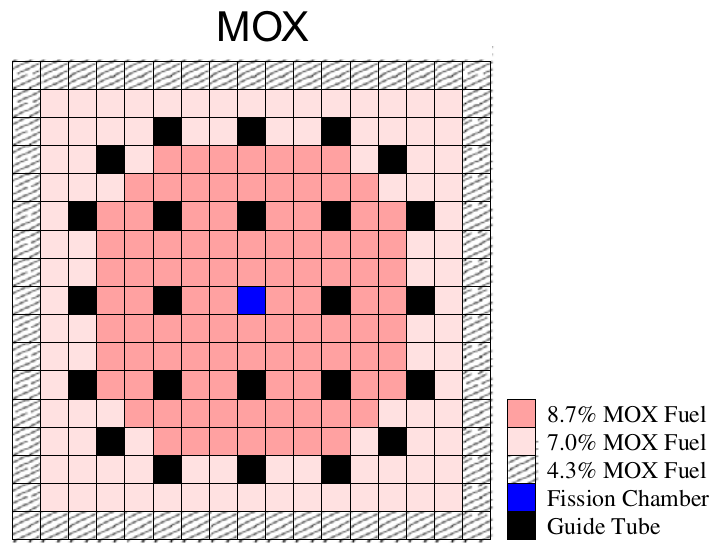
\includegraphics[width=0.95\linewidth]{figures/bench-config3.png}
    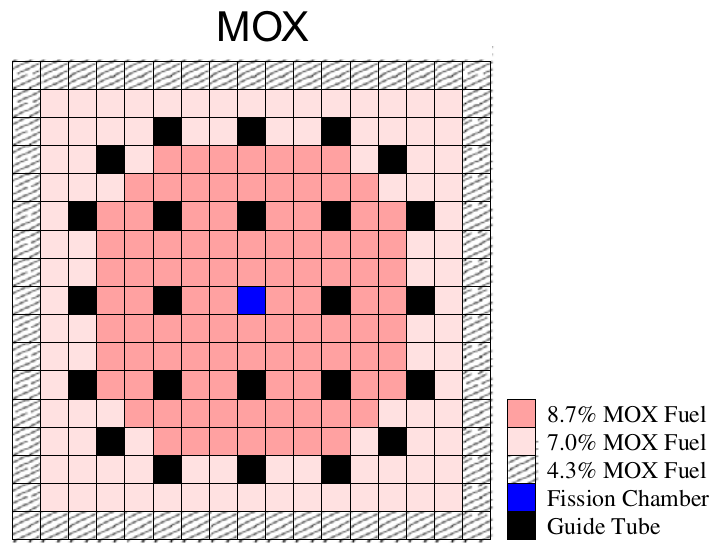
\includegraphics[trim=0 0 0 2.1cm, clip=true, width=0.85\linewidth]{figures/bench-config3.png}
    \hfill
    \caption{Structure of the MOX assembly. Image reproduced from \cite{capilla_applications_2009}.}
    \label{fig:bench3}
\end{figure}

For the sake of comparison, we conducted the exercise with and without the transport correction for calculating $D_{0,g}$ with equations \ref{eq:diff-tr} and \ref{eq:diff-rem}, respectively.
Due to the problem's symmetry, the model included only a quarter of the core.
The mesh had $2.4 \times 10^{4}$ elements.
The simulation convergence criterion was $10^{-8}$ for the neutron flux.

Table \ref{tab:keff-2nd} compares the eigenvalues obtained with the SP$_3$ solver and the references.
For the method without correction, we used an eigenvalue reference value from Capilla et al. \cite{capilla_applications_2009} as they conducted the exercise without correction.
For the method with transport correction, we used the reference value from the benchmark \cite{cavarec_benchmark_1994}.
% \usepackage{booktabs}
\begin{table}[htbp!]
	\centering
	\caption{Comparison between the results obtained with the SP$_3$ solver using no correction (equation \ref{eq:diff-rem}), the transport correction (equation \ref{eq:diff-tr}), and the reference results for the C5 MOX Benchmark.}
	\label{tab:keff-2nd}
	\begin{tabular}{lrrr}
	\toprule
							& $k_{Ref}$ & $k_{SP_3}$	& $\Delta_{\rho}$	\\
	\midrule
	No correction			& 0.96969	& 0.97106		& 145				\\
	Transport correction	& 0.93755	& 0.93792		& 43				\\
	\bottomrule
	\end{tabular}
\end{table}

% discussion about the transport correction
The results obtained with the SP$_3$ solver are within 145 pcm of the reference values.
However, the difference between the reference values of the different schemes is 3535 pcm, suggesting that the use of the transport correction is necessary.
% examples of codes using the diagonal transport correction PARCS \cite{downar_parcs_2004}, DYN3D \cite{beckert_development_2007}

% Pin-by-pin power distribution: choose one of the 3, the one w/ largest errors

The next step was to calculate the pin power distribution.
Figure \ref{fig:power-pbp} shows the relative difference to the reference provided by the benchmark \cite{cavarec_benchmark_1994} of the pin power distribution calculated with Cerberus in the MOX assembly located in the lower right of Figure \ref{fig:bench1}.
We present this result for the MOX assembly only, as it has the largest relative errors.
The largest relative error is 1.88\%.
For conciseness, we only calculated the power distribution using the transport correction.

\begin{figure}[h] %or H 
    \centering
    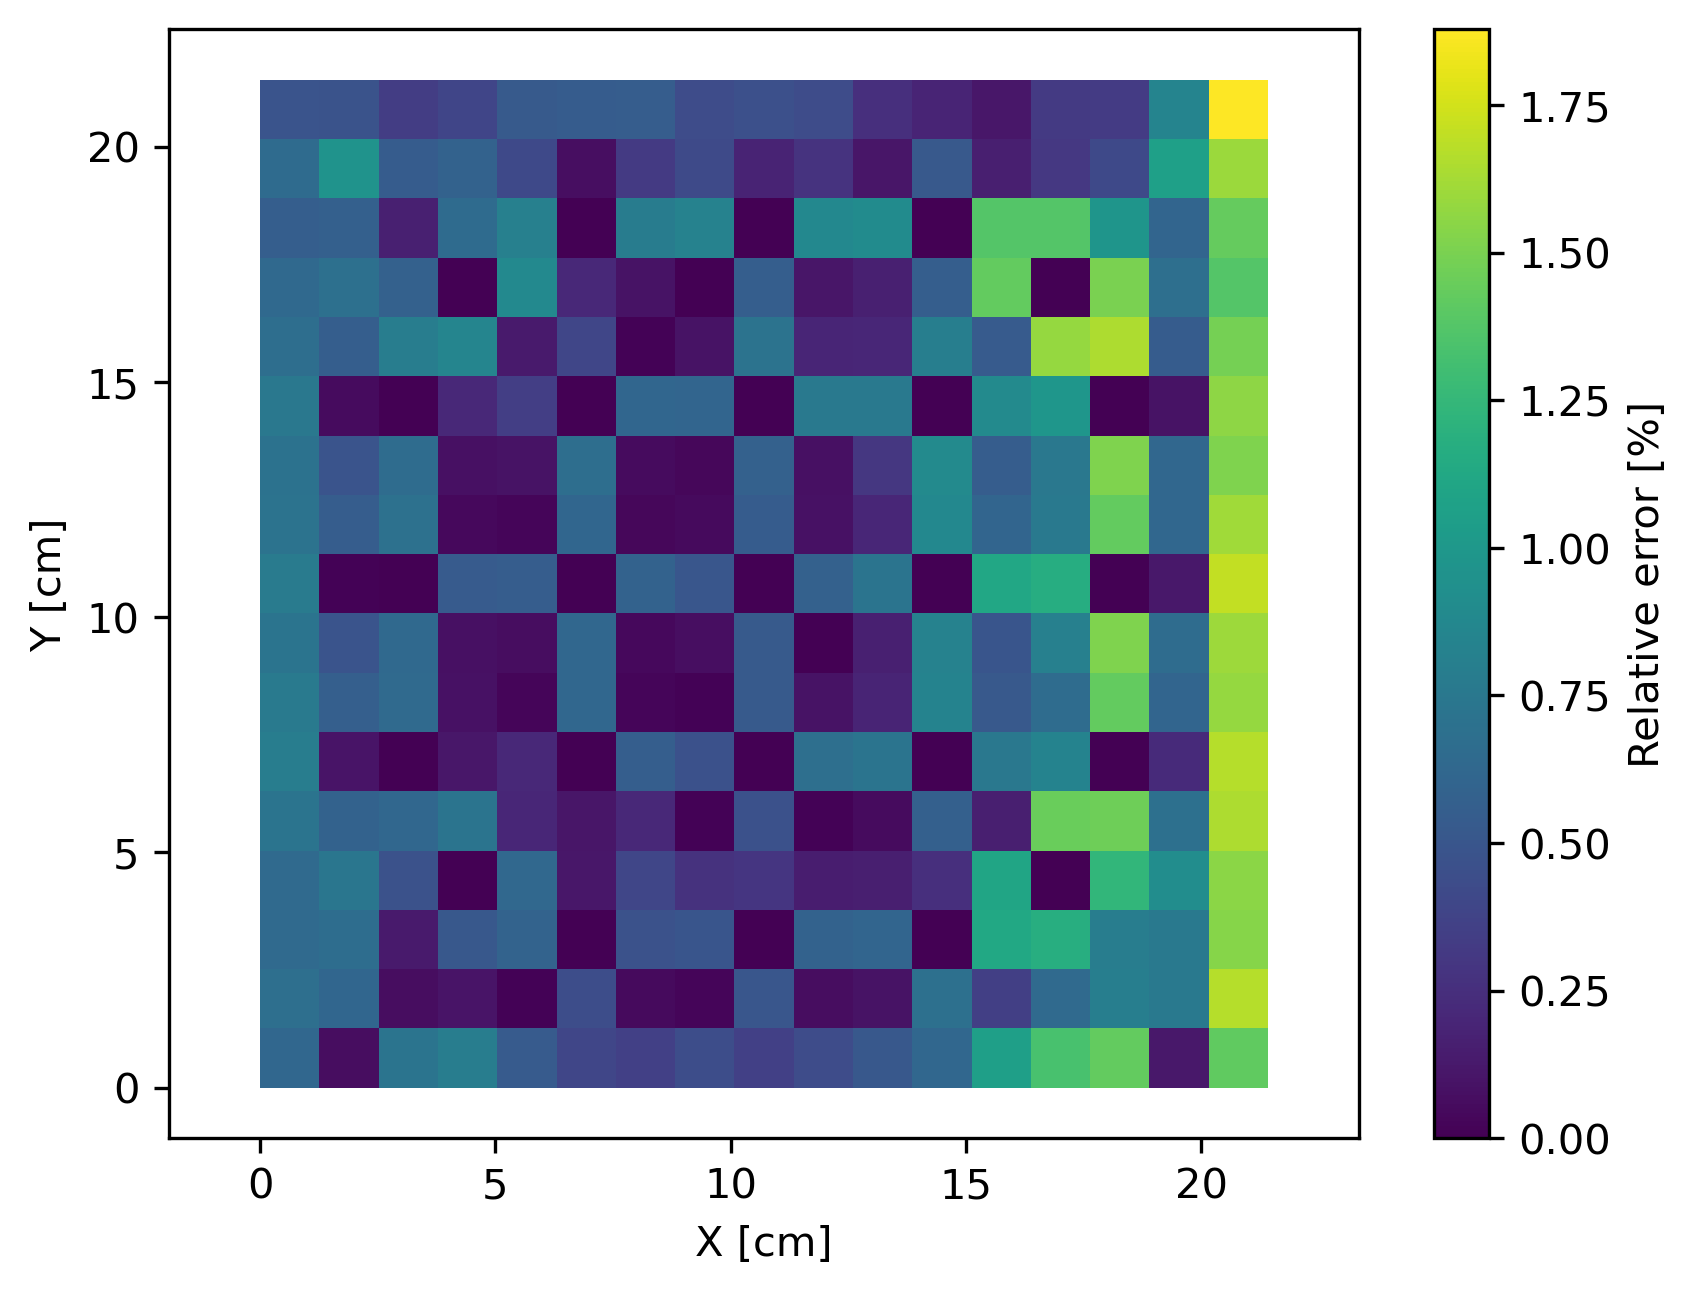
\includegraphics[width=0.85\linewidth]{figures/mox-r-pin-by-pin.png}
    \hfill
    \caption{Power distribution in the MOX assembly of the C5 MOX Benchmark.}
    \label{fig:power-pbp}
\end{figure}

% \subsection{Comparison to Diffusion solver}
% Comparison w/ Moltres, keff and neutron flux

% \begin{figure}[htbp!] %or H 
%     \centering
%     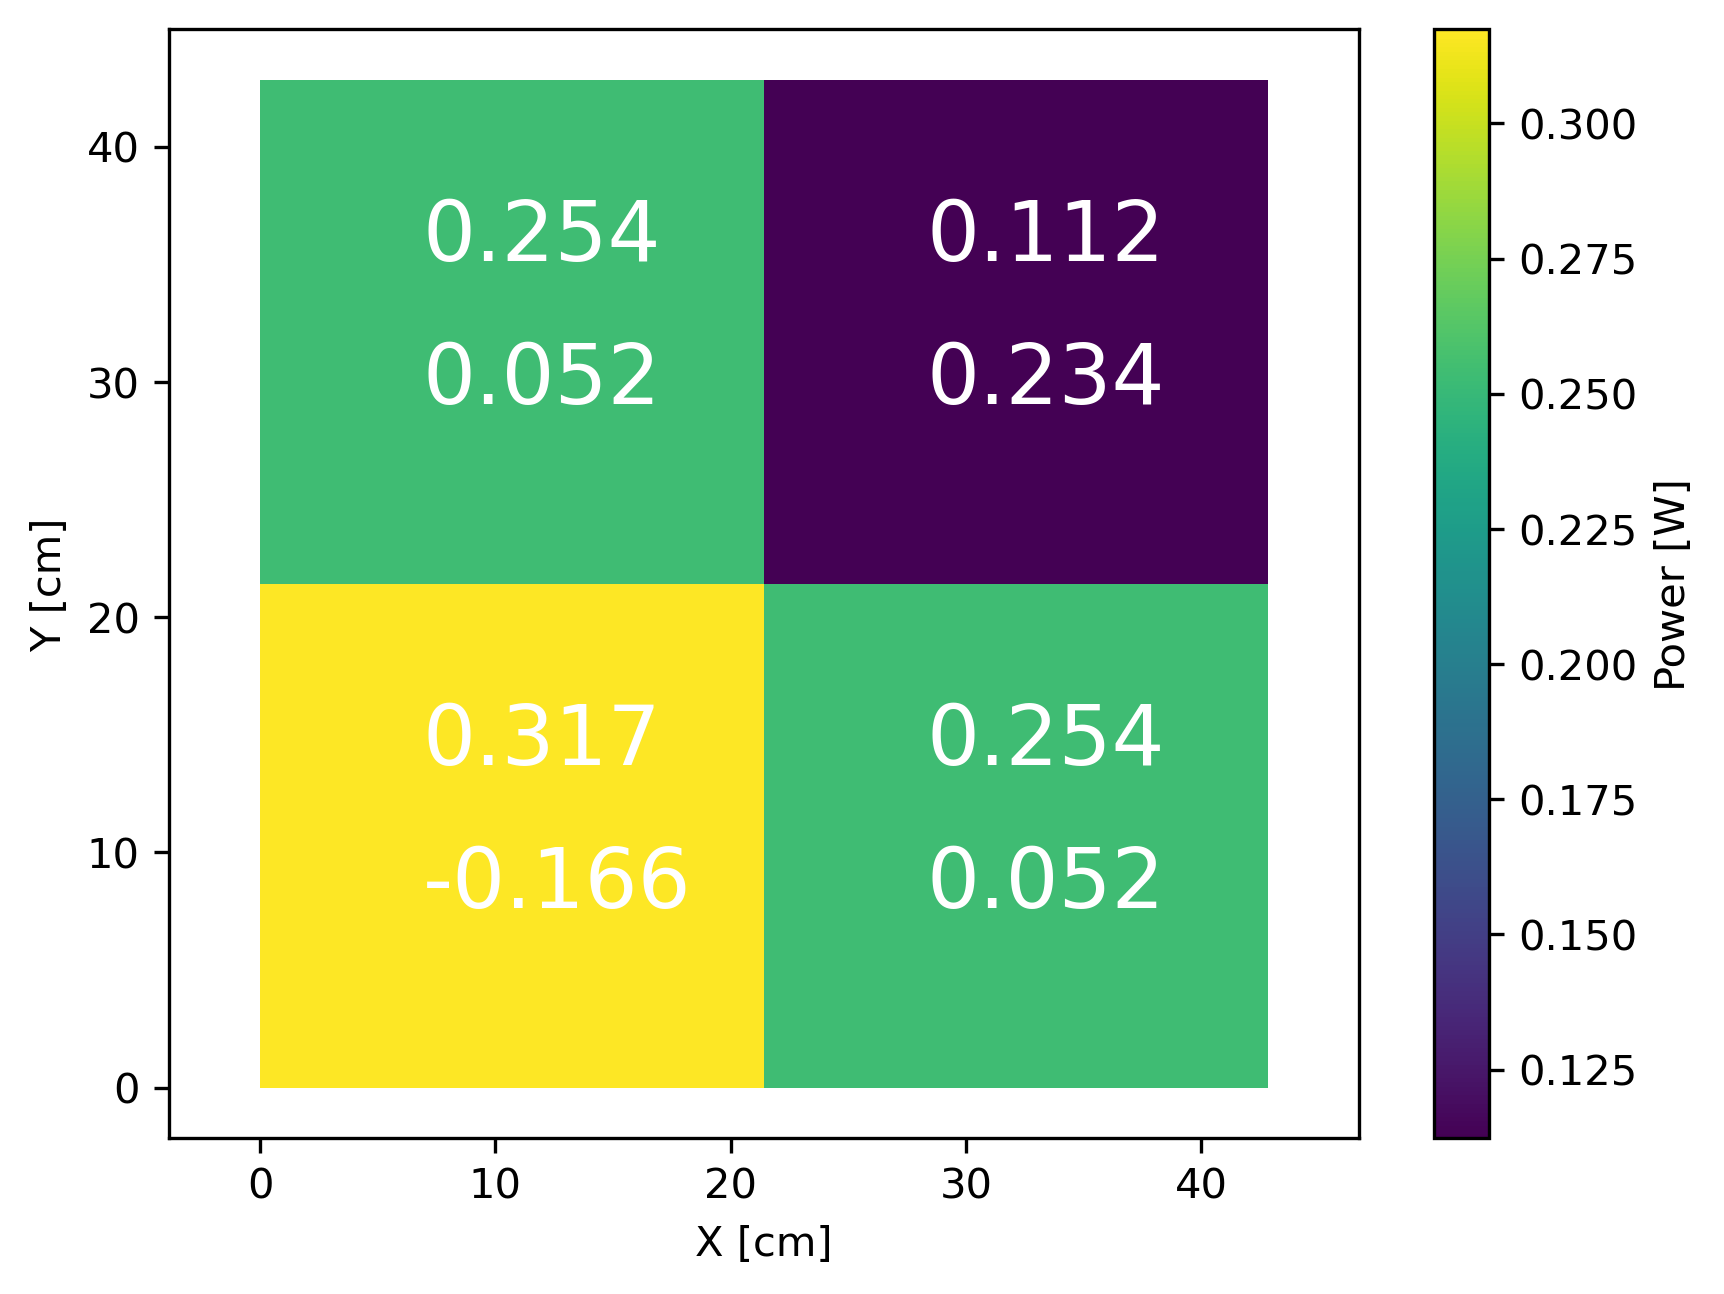
\includegraphics[width=0.95\linewidth]{figures/distrib.png}
%     \hfill
%     \caption{Power distribution in the C5 MOX Benchmark. Top: power distribution. Bottom: relative difference to reference values expressed in \%.}
%     \label{fig:power-distrib}
% \end{figure}



\section{C5G2 3D Benchmark}

% intro: exercise description
\cite{lewis_benchmark_2001}

\cite{ryu_finite_2013}


% geometry description

Figure \ref{fig:c5g2-3d} displays the axial layout of the core.

\begin{figure}[h] %or H 
    \centering
    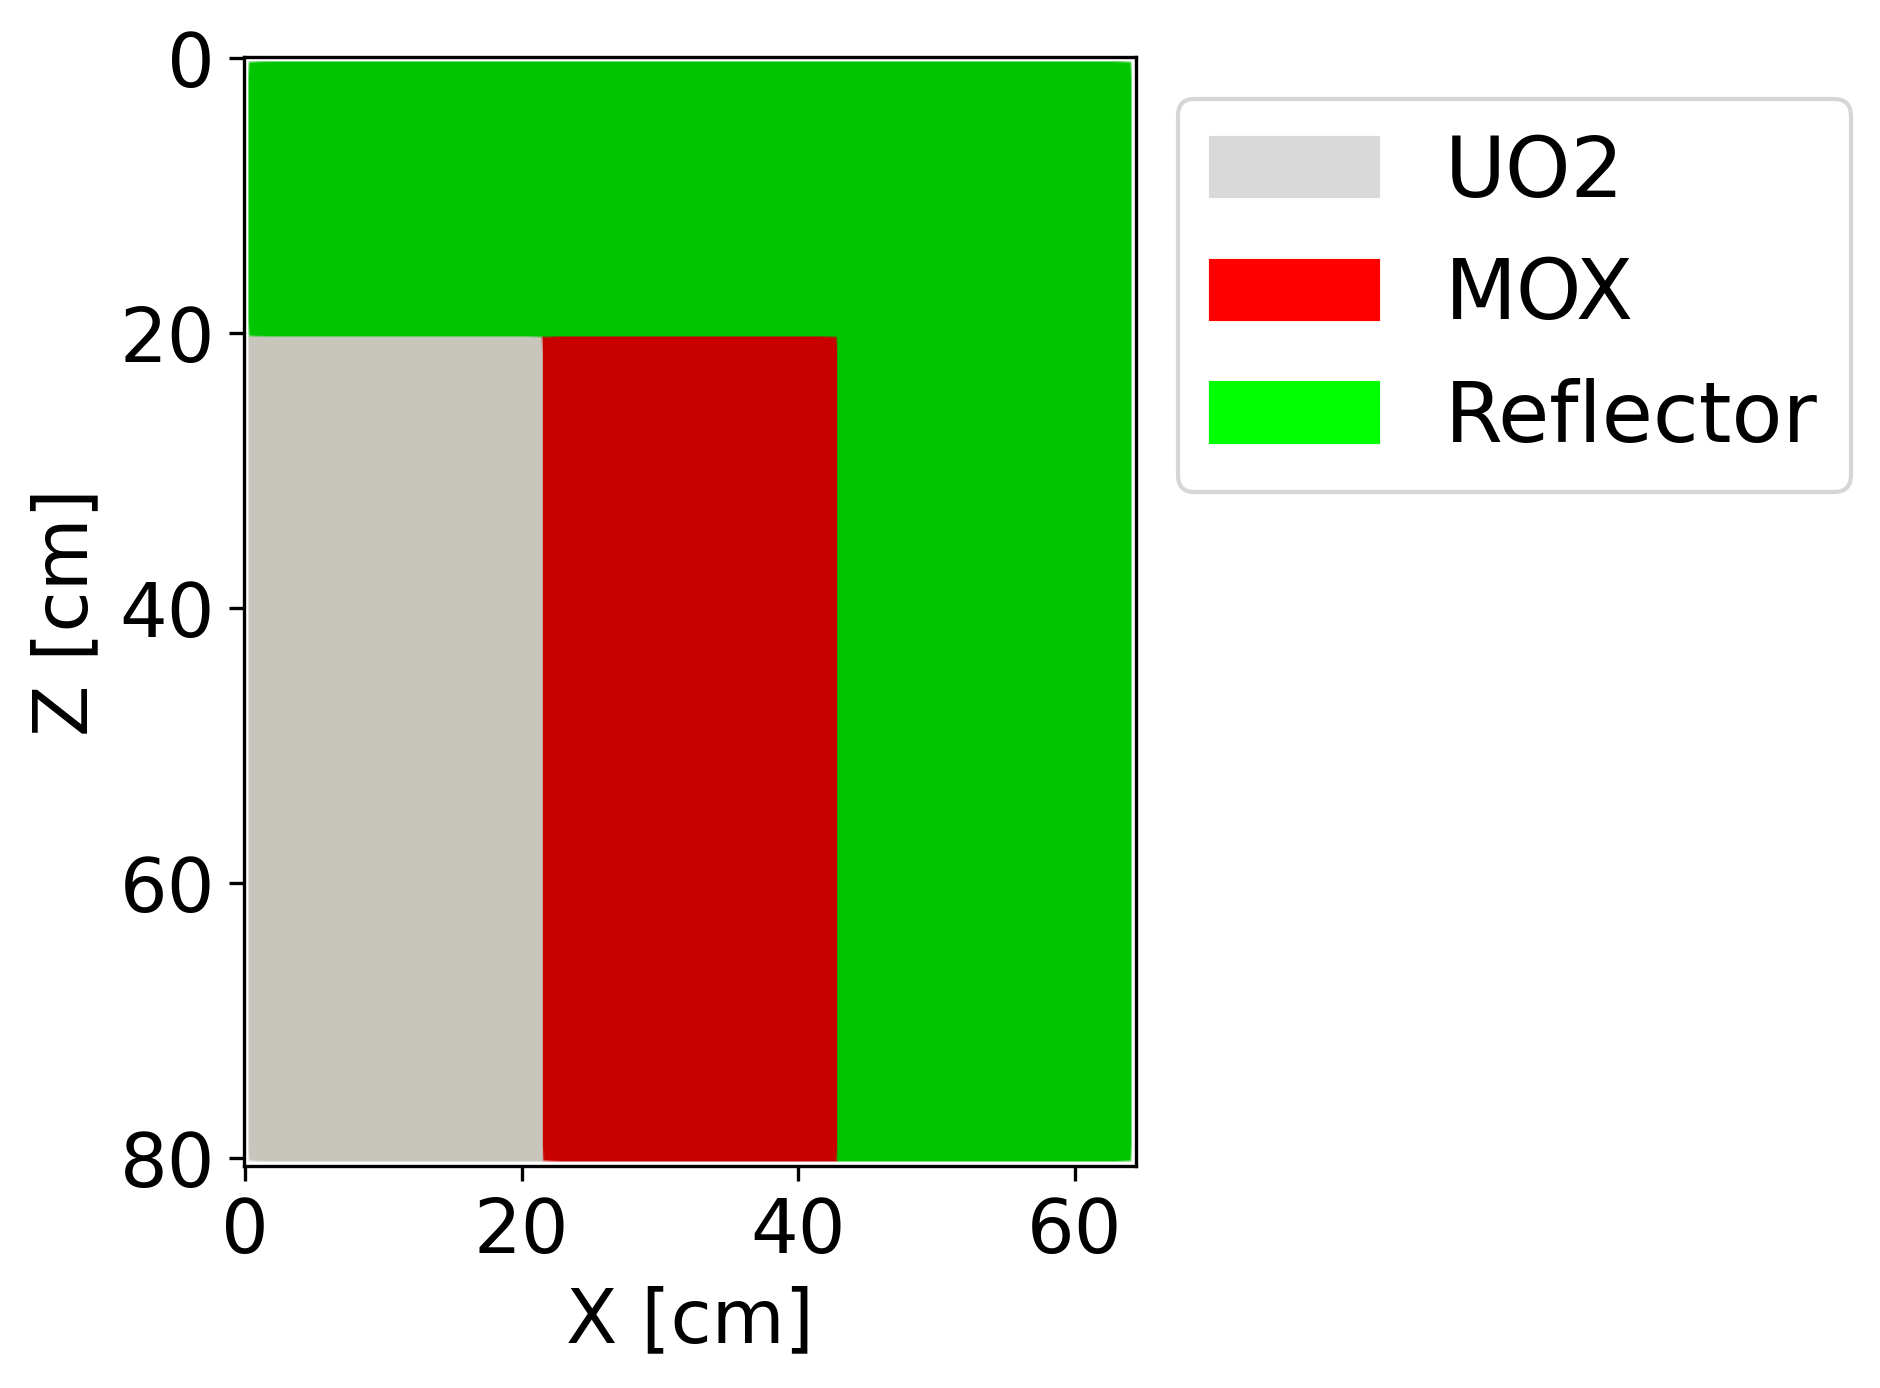
\includegraphics[width=0.85\linewidth]{figures/geo-xz2.png}
    \hfill
    \caption{.}
    \label{fig:c5g2-3d}
\end{figure}

% cross-section description
Where did they come from?



% Results comparison
Table \ref{tab:keff-4th} ...

\begin{table}[htbp!]
    \centering
    \caption{Comparison between the result obtained with Cerberus and the reference result for the C5G2 3D benchmark problem in \cite{ryu_finite_2013}.}
    \label{tab:keff-4th}
    \begin{tabular}{lll}
    \toprule
        $k_{Ref}$   & $k_{SP_3}$    & $\Delta_{\rho}$   \\
    \midrule
        0.91974     & 0.91979       & 6                 \\
    \bottomrule
    \end{tabular}
\end{table}

% Power distribution Figure
Figure \ref{fig:c5g2-3d-power}

\begin{figure}[h] %or H 
    \centering
    \includegraphics[width=0.85\linewidth]{figures/C5G2-distrib.png}
    \hfill
    \caption{.}
    \label{fig:c5g2-3d-power}
\end{figure}




\section{Conclusions}

MOOSE is a computational framework that solves systems of nonlinear differential equations.
As part of this work, we implemented the kernels to solve the steady-state SP$_3$ equations in a MOOSE-based application.
Additionally, we carried out two exercises whose reference results were known.
The first exercise solved a one-group eigenvalue problem with a simple geometry, with a result within the 12 pcm.
The second exercise studied the C5 MOX Benchmark, solving it using different approaches and obtaining results within the 145 pcm.
The calculated power distribution values were within the 1\% error from the reference.

While the SP$_3$ equations solve the neutronics in a nuclear reactor, future work may develop other applications to solve the thermal-fluids or integrate this application to existing applications.
MOOSE-based applications share the same API making their integration straightforward.


\section{Acknowledgements}

This research is being performed using funding received from the DOE Office of Nuclear Energy's University Program (Project 20-19693, DE-NE0008972) 'Evaluation of micro-reactor requirements and performance in an existing well-characterized micro-grid'.
Prof. Huff is also supported by the Nuclear Regulatory Commission Faculty Development Program (award NRC-HQ-84-14-G-0054 Program B), the Blue Waters sustained-petascale computing project supported by the National Science Foundation (awards OCI-0725070 and ACI-1238993) and the state of Illinois, the DOE ARPA-E MEITNER Program (award DE-AR0000983), and the DOE H2@Scale Program (Award Number: DE-EE0008832).

%%%%%%%%%%%%%%%%%%%%%%%%%%%%%%%%%%%%%%%%%%%%%%%%%%%%%%%%%%%%%%%%%%%%%%%%%%%%%%%%
\bibliographystyle{ans}
\bibliography{bibliography}
\end{document}

% \begin{figure}[htbp!] %or H 
%     \centering
%     \includegraphics[width=0.95\linewidth]{figures/radial-layout.png}
%     \hfill
%     \caption{Core radial layout. Image reproduced from \cite{oecd_nea_benchmark_2017}.}
%     \label{fig:radial}
% \end{figure}

% \begin{align}
%     \frac{1}{v_g}\frac{\partial}{\partial t} \phi_g &= \nabla \cdot D_g
%     \nabla \phi_g - \Sigma_g^r \phi_g \sum_{g \ne g'}^G
%     \Sigma_{g'\rightarrow g}^s \phi_{g'} \label{eq:diffusion}
%     \intertext{where}
%     C_i &= \mbox{concentration of delayed neutron precursors} \notag \\
%     &\phantom{{}=1} \mbox{in precursor group $i$}.
% \end{align}
